\documentclass[a4paper,12pt]{article}
\usepackage{titling}
\usepackage{lscape}
\usepackage{amssymb, amsmath, amssymb}
\usepackage{booktabs}
\usepackage{makecell}
\usepackage{float}
\floatplacement{figure}{H}
\usepackage[stable]{footmisc}
\usepackage{lmodern}
\usepackage{microtype}
\usepackage{libertine}
\usepackage[libertine]{newtxmath}
\usepackage[scale=.8]{FiraMono}
\usepackage[usenames, dvipsnames]{xcolor}
\usepackage{setspace}
\usepackage{float}
\usepackage[top=2cm, bottom=2cm, left=2cm, right=2cm]{geometry}
\usepackage{graphicx}
\usepackage{xcolor}
\definecolor{darkblue}{rgb}{0.0,0.0,0.55}
\usepackage{dcolumn}
\usepackage{mathtools}
\usepackage{caption}
\usepackage[UKenglish]{babel}
\usepackage[UKenglish]{isodate}
\usepackage[authoryear]{natbib}
\usepackage{babelbib}
\cleanlookdateon
\exhyphenpenalty=10000
\hyphenpenalty=10000
\widowpenalty=10000
\clubpenalty=10000
\setcitestyle{aysep={}} 
\usepackage{etoolbox}
\makeatletter
\patchcmd{\NAT@citex}
	  {\@citea\NAT@hyper@{%
		 \NAT@nmfmt{\NAT@nm}%
		 \hyper@natlinkbreak{\NAT@aysep\NAT@spacechar}{\@citeb\@extra@b@citeb}%
		 \NAT@date}}
	  {\@citea\NAT@nmfmt{\NAT@nm}%
	   \NAT@aysep\NAT@spacechar\NAT@hyper@{\NAT@date}}{}{}
	\patchcmd{\NAT@citex}
	  {\@citea\NAT@hyper@{%
		 \NAT@nmfmt{\NAT@nm}%
		 \hyper@natlinkbreak{\NAT@spacechar\NAT@@open\if*#1*\else#1\NAT@spacechar\fi}%
		   {\@citeb\@extra@b@citeb}%
		 \NAT@date}}
	  {\@citea\NAT@nmfmt{\NAT@nm}%
	   \NAT@spacechar\NAT@@open\if*#1*\else#1\NAT@spacechar\fi\NAT@hyper@{\NAT@date}}
	  {}{}
\makeatother
\usepackage[hyphens]{url}
\usepackage[hidelinks]{hyperref}

\hypersetup{
	pdftitle={Do Elites Support Polycentric Climate Governance?},
	pdfauthor={Danilo Freire, Umberto Mignozzetti, and David Skarbek},
	pdfsubject={Climate change governance},
    pdfkeywords={climate change, conjoint experiment, elites, Latin America, polycentrism},
	pdfborder={0 0 0},
	breaklinks=true,
	linkcolor=Mahogany,
	citecolor=Mahogany,
	urlcolor=darkblue,
	colorlinks=true} %

\doublespacing

\title{Do Elites Support Polycentric Climate Governance? Evidence from Latin American Countries\thanks{We thank Nigel Ashford, F\'{a}bio Barros, Daniel D'Amico, Malte Hendricks, Christian H\"{u}bner, Karina Marzano, Emily Skarbek, and Matias Spektor for helpful and engaging feedback. This research received financial support from the Konrad Adenauer Stiftung Latin American Regional Programme for Energy Security and Climate (EKLA-KAS). The authors declare there are no conflicts of interest. The data, code, and any additional materials required to replicate all analyses in this article are available at \href{http://github.com/danilofreire/climate-governance}{\texttt{http://github.com/danilofreire/climate-governance}}.}}

\author{Danilo Freire\thanks{Postdoctoral Research Associate, The Political Theory Project, Brown University, Providence, RI 02912, USA, \href{mailto:danilo_freire@brown.edu}{\texttt{danilo\_freire@brown.edu}}, \href{http://danilofreire.github.io}{\texttt{http://danilofreire.github.io}}, \href{http://twitter.com/danilofreire}{\texttt{http://twitter.com/danilofreire}}, Voice: +1 (401) 584-2494. Corresponding author.} 
\and Umberto Mignozzetti\thanks{School of International Relations, Funda\c{c}\~{a}o Getulio Vargas, S\~{a}o Paulo, SP, Brazil and Wilf Family Department of Politics, NYU, NY, USA, \href{mailto:umberto.mig@nyu.edu}{\texttt{umberto.mig@nyu.edu}}, \href{http://umbertomig.com}{\texttt{http://umbertomig.com}}, \href{http://twitter.com/umbertomig}{\texttt{http://twitter.com/umbertomig}}.} \and David Skarbek\thanks{The Department of Political Science and the Political Theory Project, Brown University, Providence, RI, USA, \href{mailto:david_skarbek@brown.edu}{\texttt{david\_skarbek@brown.edu}}, \href{http://davidskarbek.com}{\texttt{http://davidskarbek.com}}, \href{http://twitter.com/davidskarbek}{\texttt{http://twitter.com/davidskarbek}}.}
}

\date{\today}

\begin{document}
\maketitle

\begin{abstract}
\onehalfspacing
\noindent
Policy makers generally assume that climate change mitigation requires global scale governance. In contrast, recent studies suggest that polycentrism provides an effective alternative to top-down environmental policies. But despite the high social costs each solution implies, it is unclear which institutional arrangement potential veto players support. Here we run a conjoint experiment with elite members of 10 Latin American countries and ask respondents to evaluate 6,000 possible climate change agreements. We find that institutional features have a substantial effect on support for climate treaties. Latin American elites prefer multilevel solutions to tackle global warming, but there is considerable heterogeneity across countries and elite types. Our results identify possible challenges in crafting regional climate mitigation policies and offer new insights on how to integrate interventions at the local and international levels.

\vspace{.5cm}

\noindent 
\textbf{Keywords:} climate change, conjoint experiment, elites, Latin America, polycentrism

\vspace{.5cm}

\noindent 
\textbf{Word count:} 3,524
\end{abstract}

\newpage

\doublespacing

\section{Introduction}%
\label{sec:introduction}

Over the last years, we have seen an emerging consensus about the causes and consequences of anthropogenic climate change. Despite some variation in climate risk beliefs, mostly due to cultural worldviews and political orientation \citep{hornsey2016meta}, recent surveys show that the public is increasingly aware of the dangers of greenhouse gas emissions. For example, 59\% of Americans are sure the Earth's temperature is increasing \citep{stanfordearth2018}; 74\% of European Union citizens consider global warming a `very serious problem' \citep{europe2018survey}; and 90\% of Brazilians believe climate change is already harming people around the world \citep{pew2018climate}.

Yet this consensus does not translate itself into effective political action. Global climate negotiations have progressed slowly under the guidelines of the United Nations Framework Convention on Climate Change (UNFCCC), and there is wide scepticism that multilateral talks will move faster in the next years \citep{cole2015advantages, hjerpe2015views}. As carbon dioxide emissions continue to increase, current efforts are likely to be insufficient to meet the Paris Agreement target of $2^{\circ}$C temperature rise above pre-industrial levels \citep{jordan2015emergence}. Existing research affirms that this unsatisfactory performance is partially due to institutional design \citep{ostrom2014polycentric, cole2015advantages}. For instance, multilateral forums downplay the domestic constraints political leaders experience when implementing strategies to reduce greenhouse gas emissions \citep{rayner2010eat}. Universal binding agreements also offer limited scope for experimentation, which hinders the ability for individuals to solve complex collective action problems \citep{de2014global}.

Recently, scholars have argued that polycentric approaches provide a better \textit{institutional fit} for natural resource systems \citep{turnheim2018innovating, berkhout2003negotiating, carlisle2017polycentric, ostrom1990governing}. Polycentrism is defined as a political arrangement in which formally independent units operating at different levels engage in a continuous process of cooperation and competition \citep{cole2015advantages, aligica2013co}. Experiences such as inshore fisheries in Turkey and timber management in Switzerland show that polycentrism induces individual cooperation and allows communities to avoid the \textit{tragedy of the commons}, that is, the overexploitation of shared resources \citep{hardin1968tragedy, ostrom1990governing}. Authors also point out that polycentric systems improve accountability as decentralisation reduces rent-seeking opportunities for politicians and interest groups \citep{turnheim2018innovating, ostrom2012nested, ostrom2014polycentric, sovacool2013adaptation}. 

Despite the potential advantages of polycentric arrangements, two challenges may undermine their efficiency and popular support. First, polycentric systems demand constant civic participation at multiple government levels. Because climate change has diffuse benefits but concentrated costs, individuals have few incentives to join collective efforts \citep{barrett2003increasing, heitzig2011self, nordhaus2015climate}. Second, individuals tend to heavily discount climate change investments \citep{dasgupta2008discounting, nordhaus1997discounting}. Reducing carbon emissions requires significant expenditures today, yet the benefits of climate mitigation will arise only in a distant future. In that regard, citizens might prefer state-based initiatives to prevent climate change if private costs are too high or expected results too uncertain. 

Voluntary environmental governance faces further difficulties in new democracies. In Latin America, authoritarian regimes discouraged civil participation and reduced social capital, two necessary conditions for effective polycentric arrangements \citep{aligica2014institutional,ostrom1990governing}. Top-down climate policies also create incentives for organised groups to collude with state officials and pursue private interests \citep{aklin2013understanding,aklin2014blames}. As a result, elites and state representatives have \textit{de facto} veto power over environmental legislation and can override local decisions to their own benefit.

We design an experiment to assess which climate change governance system Latin American elites are willing to support. In our survey, we asked 654 respondents -- academics, members of the executive power, legislators, businesspeople, and members of non-governmental organisations -- to select their preferred agreement in 7 randomised binary choices.

In what follows, we describe our experimental methods and results. We then turn to two additional analyses, in which we disaggregate the responses according to country and elite type, and proceed to the concluding remarks.

\section{Data and Methods}%
\label{sec:data_and_methods}

We use conjoint experiments to estimate the effect of institutional features on climate mitigation agreements. Our sample consists of Latin American elites. Latin America is the most biodiverse region in the world and plays a major role in global climate mitigation projects. For instance, the Amazon basin contains about half of the world's carbon stock, so local elites are essential for the success of emissions trading markets \citep{benitez2006site, yang2018post}. Second, Latin American elites have wide disagreements over preservation policies, and the recent shift towards populist governments has highlighted the need for a robust framework to protect environmental resources \citep{ellner2019pinktide, lyall2019speculative, sagarzazu2019foreign}. In that regard, veto players can counterbalance governmental time discounting and secure the long-term provision of public goods. Lastly, survey experiments on climate policies have focused on a small set of developed countries, so truly comparative experimental work remains scarce. We fill this gap by analysing 10 countries where elites have different stakes at climate change negotiations.  

We use a dataset compiled specifically for this study. From 1\textsuperscript{st} of October to 5\textsuperscript{th} of December 2018, we ran an elite survey in Argentina, Bolivia, Brazil, Chile, Colombia, Costa Rica, Ecuador, Mexico, Panama, and Peru. We started by gathering information on Latin American elites. For each country, we collected the profiles of 100 members of the Executive, 100 members of the Legislative, 150 academics in the energy sector, and 150 members of the civil society. We then sampled these profiles until we achieved a minimum of 10\% of responses within each group. We ran our survey both online and by telephone, collecting information on the climate change agreements and other related questions.

After finishing this dataset, we started the surveying stage. From 12\textsuperscript{th} of November to 5\textsuperscript{th} of December, we ran the survey by contacting elite members by phone or by email. We had two teams of enumerators, one based in S\~{a}o Paulo and another based in Rio de Janeiro, Brazil, comprised of Portuguese and Spanish native speakers. Please refer to the Supplementary Material for more information about the sampling process and descriptive statistics.

The hypothetical climate change agreements includes six attributes: 1) which organisation defines the rules; 2) how would conflicts be resolved; 3) what punishment should be applied to rule-breakers; 4) how should repeated violations be sanctioned; 5) which countries should bear the costs of the agreement; 6) how often should the agreement be renegotiated. Table~\ref{tab:categories} describes the values we included in each treaty attribute. \\

\newpage 

\begin{table}[ht]
\begin{center}
\caption{\textbf{Attributes and values for climate change mitigation conjoint experiments}}
\label{tab:categories} 
\begin{tabular}{l !{\vrule width 1pt}p{9cm}}
\Xhline{2\arrayrulewidth}
\textbf{Attribute} & \multicolumn{1}{c}{\textbf{Values}} \\
\Xhline{2\arrayrulewidth} \\
Who makes the rules? & International organisations; federal government; local government; local community members; non-governmental organisations \\
& \\
Conflict resolution mechanism & United Nations; government bureaucracy; local courts; private arbitration; informal norms \\
& \\
Punishment & Imprisonment; fines; blacklist; none \\
& \\
Punishment for repeated violations & More penalty; same; less penalty \\
& \\
Agreement costs & Rich countries pay more than poor countries; proportional to history of emissions; proportional to current emissions; only rich countries pay \\
& \\
Renegotiation & Never; fifty years; twenty years; five years; one year \\
\Xhline{2\arrayrulewidth} 
\end{tabular}
\end{center}
\end{table}

The categories map main conceptual differences between polycentric and state-led climate mitigation policies \citep[e.g.][]{bechtel2013mass, ostrom1990governing}. The conjoint experiment design opens the possibility for interviewees to combine multiple levels of governance into a single climate change agreement as they see fit. We give no prior indication of whether a certain value is more prevalent in actual agreements, and we randomise the values to ensure that they all have the same probability of being selected. In total, there are 6,000 possible value combinations. Figure~\ref{fig:conjoint} illustrates our experimental design.

\begin{figure}[H]
	\centering
	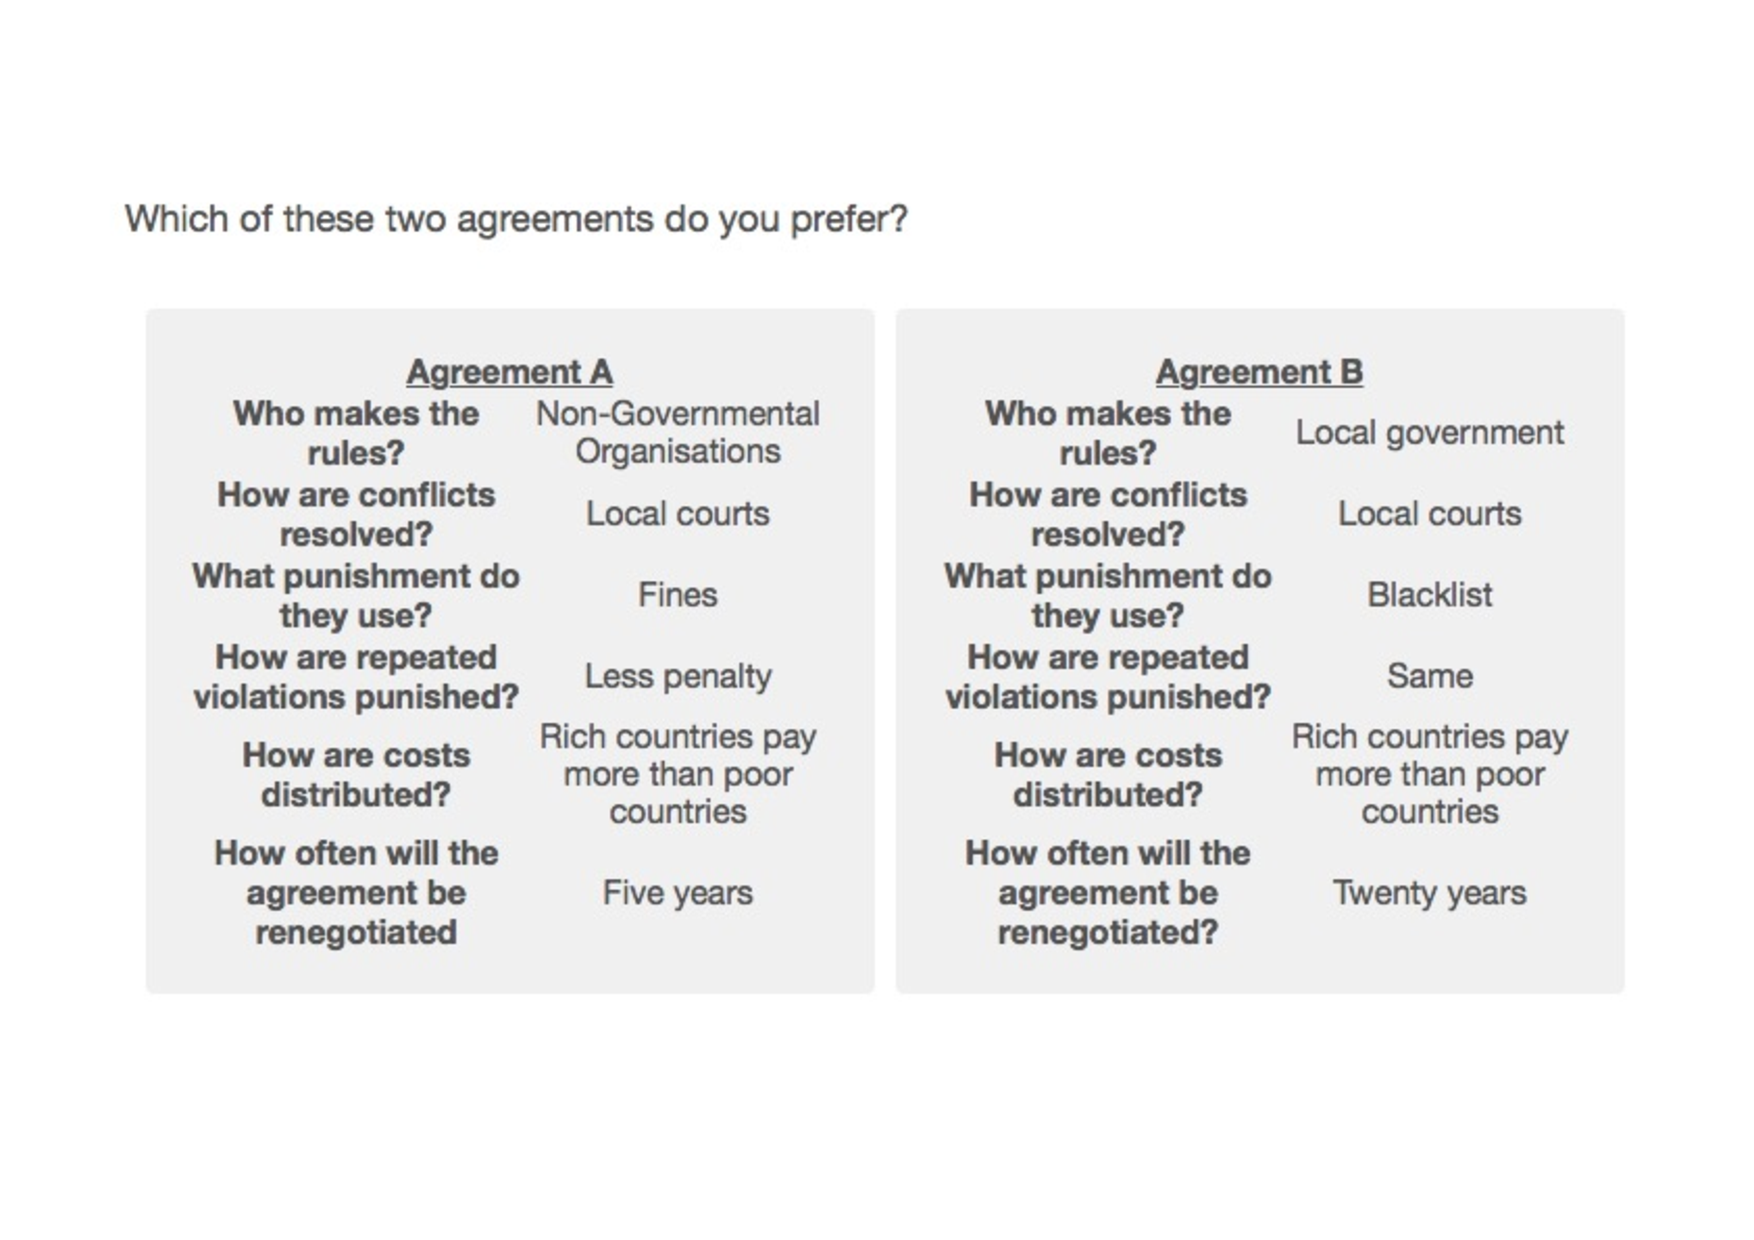
\includegraphics[width=13cm]{conjoint-cropped.pdf}
	\caption{\textbf{Example of conjoint table presented to respondents}}
	\label{fig:conjoint}
\end{figure}

We estimate our models with the \texttt{cregg} package \citep{leeper2018cregg} for the \texttt{R} statistical language \citep{rstats2019}. Here we report marginal means instead of average marginal conditional effects (AMCE) of climate agreement attributes. \citet{leeper2018subgroup} show that AMCEs can be misleading in subgroup analysis as model results are sensitive to the choice of reference categories in interactions. In contrast, marginal means provide a clear description of quantities of interest, in our case preferences towards agreement attributes, while allowing for easy comparisons between groups of respondents. For these reasons, we include marginal means in the visual presentation of our results. Readers can refer to the Supplementary Material for AMCE estimates.  

\section{Results}%
\label{sec:results}

Figure~\ref{fig:pooled} shows our main results. The graph illustrates the preference associated with each attribute of hypothetical climate mitigation agreements. Dots with horizontal bars represent point estimates and 95\% confidence intervals from linear regressions with cluster-robust standard errors. \\ 

\begin{figure}[H]
	\centering
	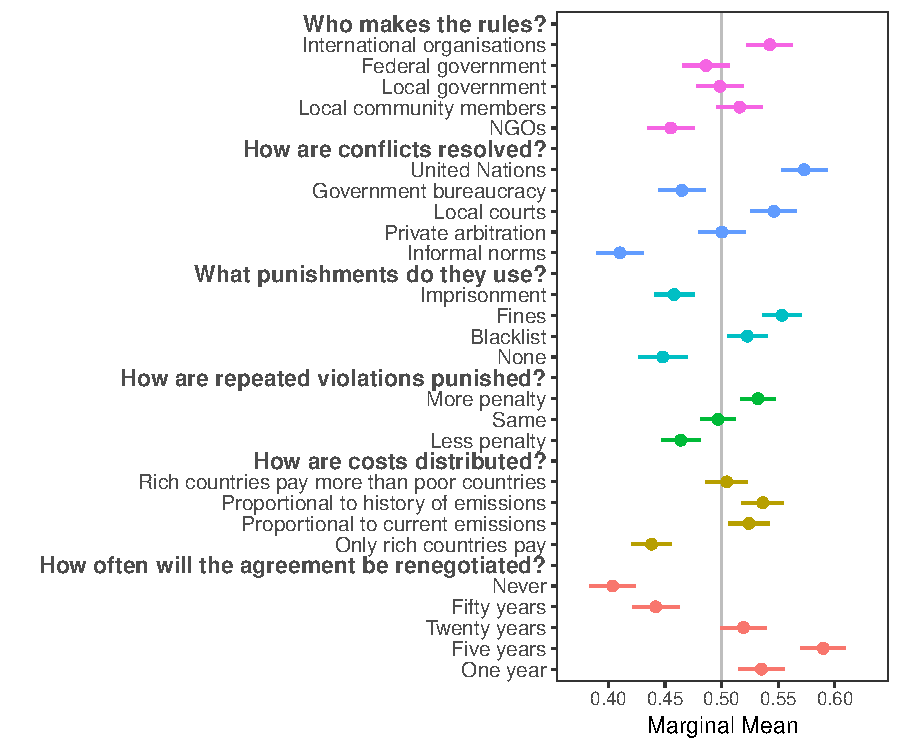
\includegraphics[width=.9\linewidth,height=11.5cm]{pooled.pdf}
	\caption{\textbf{Effect of institutional attributes on the probability of support for climate change agreements in 10 Latin American countries (pooled data)}}
	\label{fig:pooled}
\end{figure}

Respondents prefer international organisations to establish climate mitigation rules (54\%, SE = 1.2), but they also hold favourable views of local communities (51.6\%, SE = 1.25), local governments (49.8\%, SE = 1.2), and state governments (48.6\%, SE = 1.3) as rule-makers. Although local communities receive slightly more support than the other alternatives, the differences among the three groups are not statistically significant. We note that Latin American elites support multiple governance levels simultaneously, what suggests they are willing to include separate political spheres into a single climate regime. We also observe that non-governmental organisations are the least preferred option for climate change rule-making with 45.5\% (SE = 1.3). 

We see a similar pattern with respect to conflict resolution. Respondents affirm disputes should be addressed mainly by the United Nations and local courts. These two choices have 57.3\% (SE = 1.2) and 54.6\% (SE = 1.2) approval, respectively. Private arbitration comes next with 50\% (SE = 1.3), followed by government bureaucracy with 46.4\% (SE = 1.3). Informal norms receive only 41\% support (SE = 1.3). 

Participants agree with graduated sanctions to repeated offenders (53.2\%, SE = 0.9) and they believe agreement costs should be allocated according to the country's history of emissions (53.6\%, SE = 1.1). Moreover, related to the same idea of proportionality, respondents indicate that lawbreakers should be punished with fines (55.3\%, SE = 1.1), which can be easily increased if necessary.

We find no evidence that rich countries alone should bear the burden of climate change mitigation costs. Latin American elites believe developing countries should also contribute to the provision of global public goods. Our sample views it was legitimate to contribute to climate change solutions, so this may not be a major source of free riding to climate change solutions in the region.

In terms of agreement duration, respondents are interested in a balance between stability and flexibility. Interviewees reject agreements that either cannot be modified or that last for 50 years. Their preference lies in agreements that can be renegotiated every five years (59\%, SE = 1.2), as they are durable enough to provide long-term incentives to the parties, yet still adaptable to unforeseen demands.

Overall, the results do not conform to strictly top-down or bottom-down approaches. While elites favour solutions provided at the macro level, they are also open to input from other government actors and local groups. But we find little support for fully polycentric arrangements either. As we noted above, the data do not show major difference in preferences between federal and local governments and between these and community-based solutions. Further, the rejection on non-governmental organisations points to a discredit of self-governing arrangements as a means to deal with global warming. This last result is consistent with the Latin American tradition of heavier reliance on the state than on voluntary organisations.

\begin{figure}[H]
	\centering
	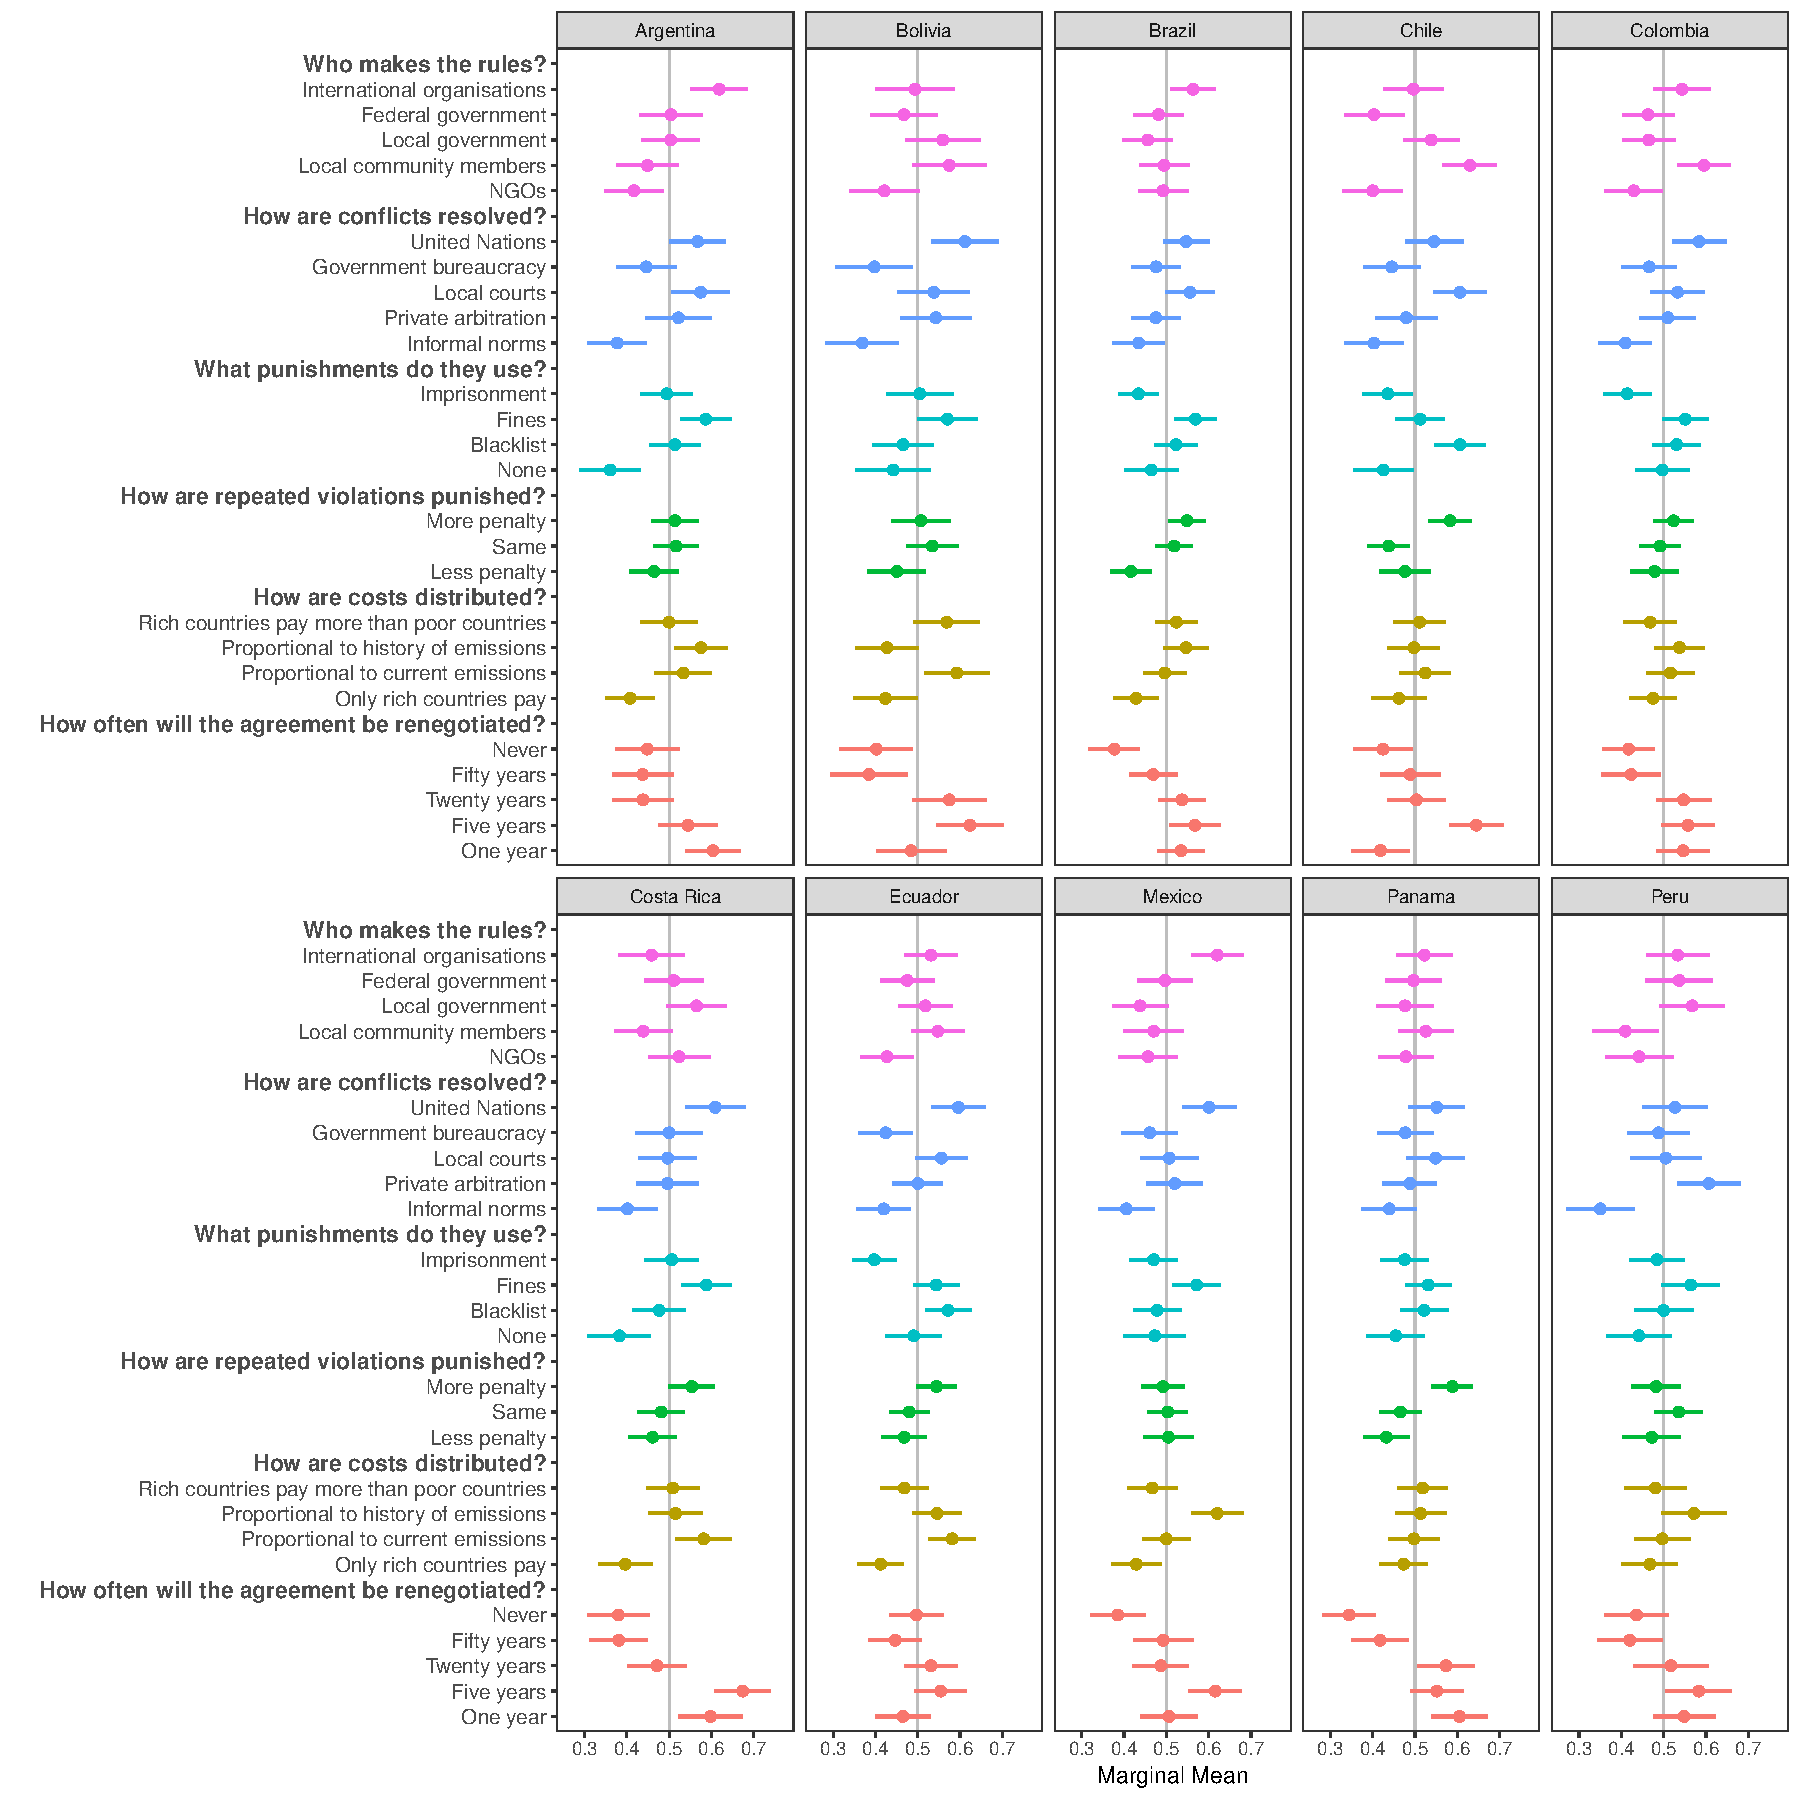
\includegraphics[width=\linewidth]{countries.pdf}
	\caption{\textbf{Effect of institutional attributes on the probability of support for climate change agreement by country}}
	\label{fig:countries}
\end{figure}

We also examine how our results vary across countries and types of elites. Figure~\ref{fig:countries} displays the preferred climate change agreement characteristics for each of the 10 countries in our sample. The disaggregated data confirm that elites have a generalised preference for a heavy role by international agencies in terms of solving conflicts, and a generalised dislike for informal norms. In addition, the cross-country results show a preference for a positive role by federal and local governments, and that local community members should also participate in the deliberation process.

However, some of the regional preferences are a by-product of sample aggregation. Latin American elites do not have a consensus on which organisations should provide the rules. For example, elites in Costa Rica prefer local to global rule-making; in Mexico, they prefer global and dislike local, similar to Peru, Argentina, and Brazil; in Colombia, elites favour global and local rule-making simultaneously; and in Bolivia, respondents prefer local organisations to design climate treaties. This is an important point and has far-reaching consequences for policy design in the region. The lack of coordination on rule-making responsibilities may configure a case of Arrow's impossibility theorem \citep{arrow1950difficulty}. Should a polycentric system be put for vote at international arenas such as the United Nations or the Organisation of American States, it is not clear how elites would reach a consensus decision. Based on our data, we cannot affirm which outcome would prevail. 

Figure~\ref{fig:types} shows the results disaggregated by elite type. Academics, members of the civil society, and representatives in the executive and legislative branches hold similar views about how conflicts should be resolved, what punishment to apply to lawbreakers (fines and blacklisting), and the duration of the agreements. These are in line with our previous results.

\begin{figure}[H]
	\centering
	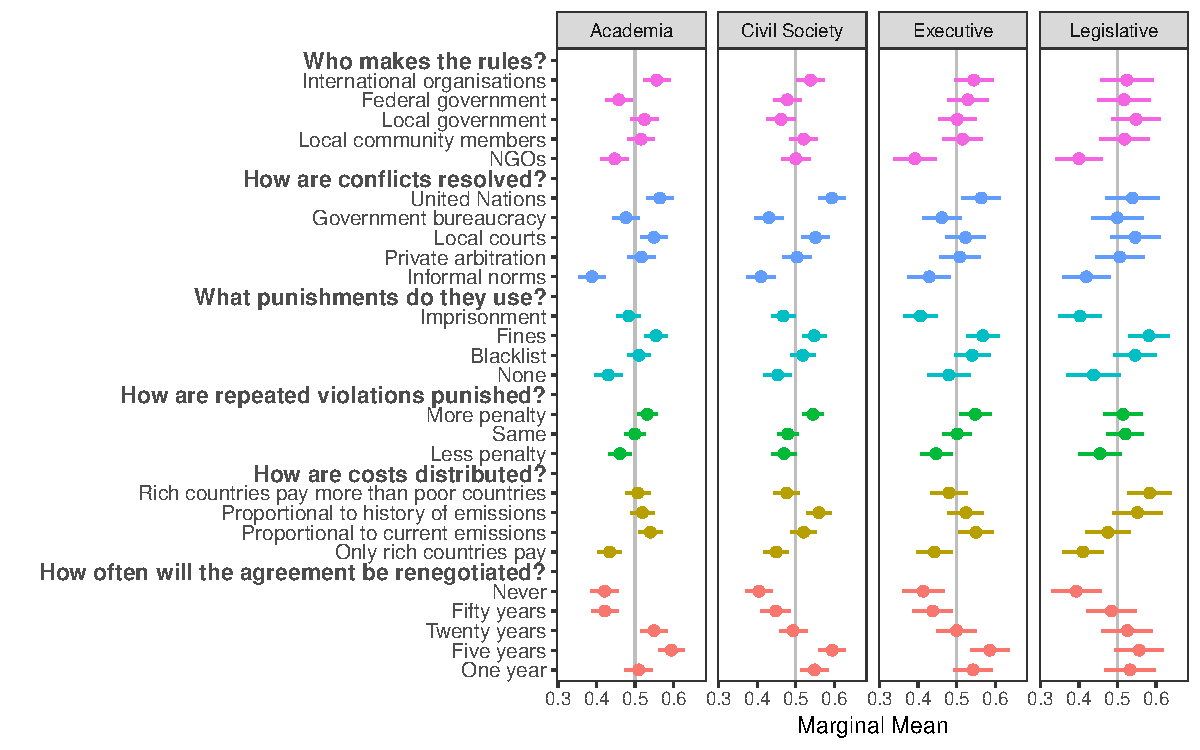
\includegraphics[width=\linewidth]{types.pdf}
	\caption{\textbf{Effect of institutional attributes on the probability of support for climate change agreement by elite type}}
	\label{fig:types}
\end{figure}

Significant differences emerge in two of the six attributes of interest. First, whereas academics and members of the civil society are less favourable to allowing the federal government to formulate the rules, members of the executive and the legislative -- part of federal government themselves -- are more likely to see themselves as the preferred rule-makers. Second, members of the legislative have a stronger opinion that rich countries should bear the larger part of the agreement costs (58.4\%, SE = 3.5). 

\section{Discussion}
\label{sec:discussion}

In this article, we examine which attributes of climate change mitigation treaties Latin American elites support. We find that interviewees prefer international organisations to resolve conflicts, are favourable to imposing increasing fines on violators and renewing agreements every five years. Survey participants are sceptical about non-governmental organisations and consistently reject informal norms as an instrument to solve disputes. Taken together, our experiment suggests that Latin American elites oppose non-governmental organisations as rule-makers and want legal punishment to agreement violators. 

While our results confirm that Latin Americans prefer the state to conduce public policy, they do not match the typical cases of centralised or polycentric climate change regimes suggested in the literature. After disaggregating the data by country and elite type, we confirm that elites prefer international organisations to resolve disputes and that federal and local sources of governance should have a say in climate agreements. However, we find large heterogeneity in the responses, with groups holding different opinions on how competences should be divided. 

Our results have important theoretical and practical implications. The findings we present here suggest there is considerable scope for new studies on global governance, specially in underrepresented regions. Our analysis can be extended to examine if the Latin American public has the same opinion on multilevel arrangements as do the elites; and if not, it would be important to know what explains the mismatch between groups. Moreover, future work may address whether other areas of scholarship which assume international-level coordination could benefit from multilevel arrangements, either state-based or not.   

The findings also highlight the importance of comparative work in experimental studies. As a region, Latin America favours results that are in line with polycentric arrangements, but we find that those preferences derive from the aggregation of heterogeneous effects. Our study indicates researchers should be cautious about the external validity of experimental studies. 

With regards to environmental policies, we provide experimental evidence that individuals have preferences that are not fully represented in current climate mitigation agreements. We identify that Latin American elites are interested in incorporating different political actors and in strengthening the role international organisations play in climate governance. Future climate negotiations can achieve better results if they take those preferences into account.

\section*{Supplementary Material}
\label{sec:supplementary}

The data, code, and any additional materials required to replicate all analyses in this article are available at \href{http://github.com/danilofreire/climate-governance}{\texttt{http://github.com/danilofreire/climate-governance}}.

\bibliographystyle{apalike}
\bibliography{references.bib}

\end{document}

